\begin{comment}
\title{parslTestbookQMCblog}
\author{Dr. Sou-Cheng Choi, Illinois Tech and SouLab, Joshua Jay Herman (QMC Development Team)}
\date{September 2025}

\maketitle
Accelerating QMCpy Notebook Tests with Parsl
\end{comment}

\subsection{Introduction}


 This provides a summary of a speedup of notebook regression testing presented in my talk at Parsl Fest, sponsored by Globus Compute, and highlights subsequent directions of the work. It is joint work with Dr. Sou-Cheng Choi at Illinois Tech and SouLab LLC. Regression testing of notebooks is massively parallel and resource intensive.

\subsection{Methodology}
 Choosing Testbook allowing them to run independently without requiring execution of the full notebooks for clarity. Then we made a test harness that we could also have Parsl execute our testbook tests since it is embarrassingly parallel.

\subsection{Results}
To determine a baseline speedup with a subset of notebooks that were tested we saw a ~2.1x speedup. After increasing our test coverage that expanded our work to look for syntax errors we see now a ~4x speedup which is consistant with our expectations. 


\begin{figure}[tbp]
\centering
\begin{subfigure}[t]{0.49\textwidth}
\centering
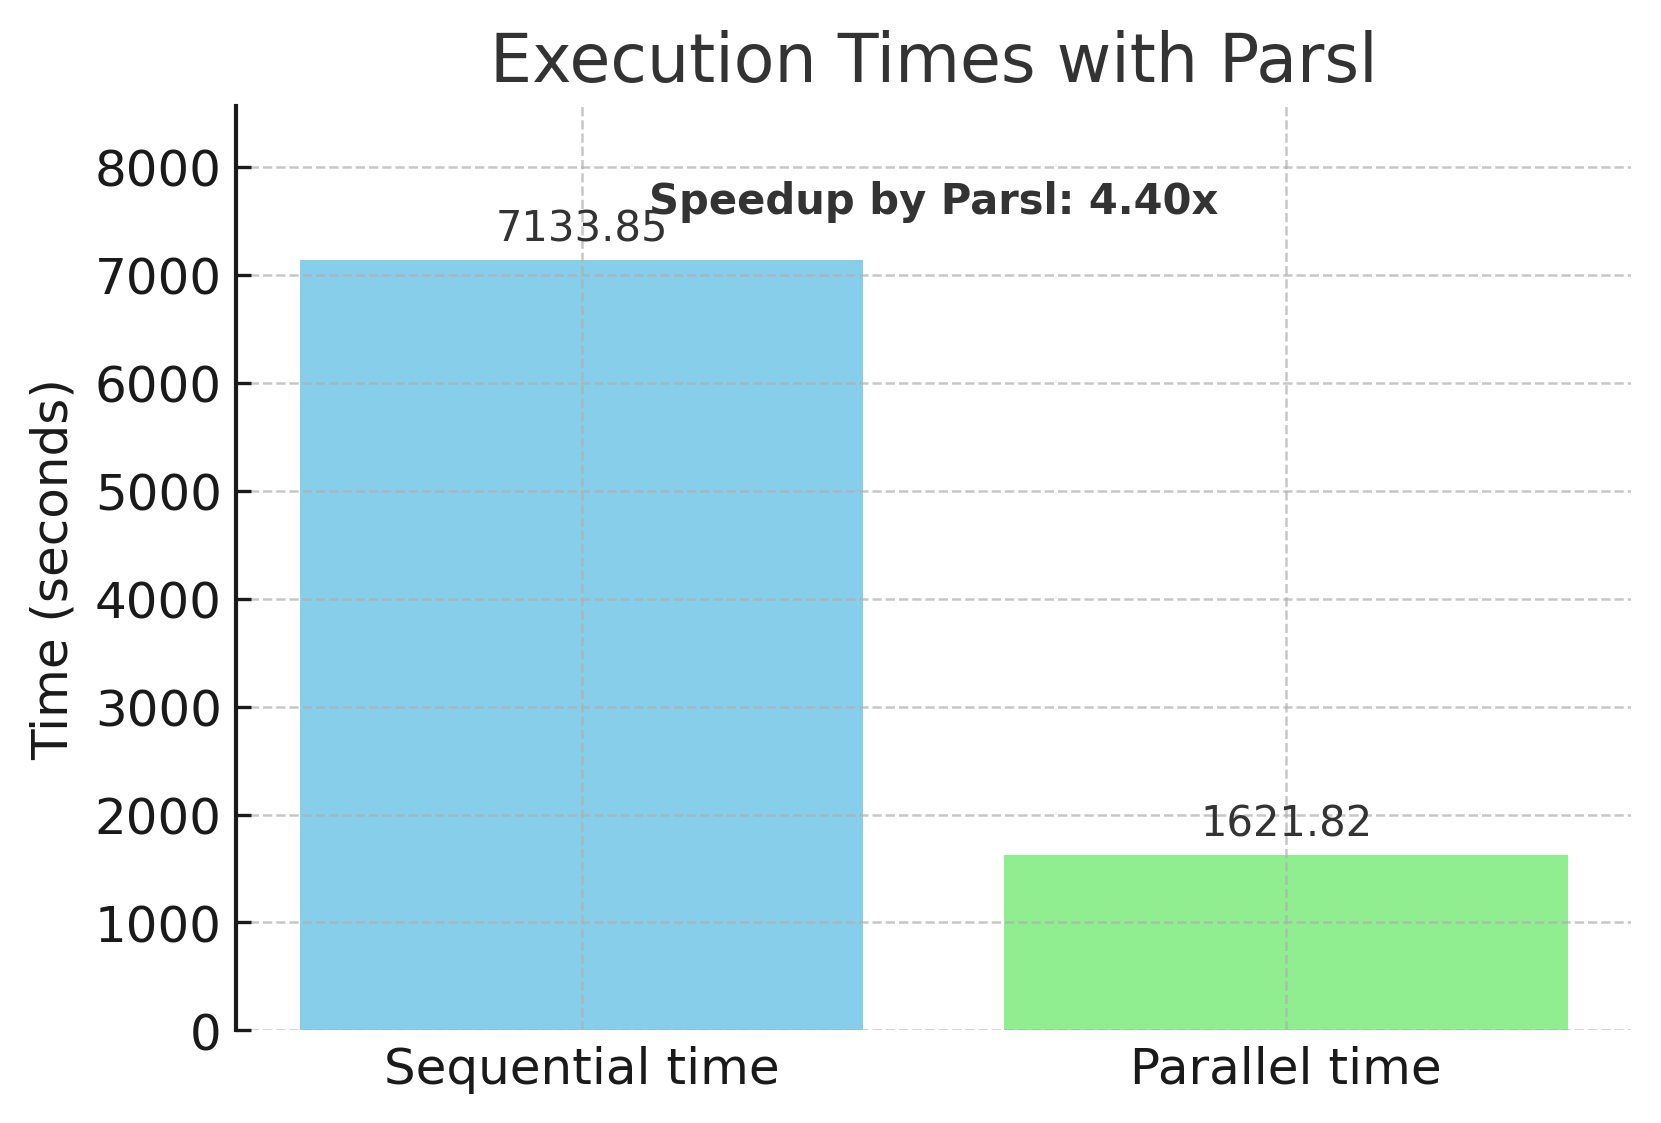
\includegraphics[width=\textwidth]{booktests/parsl_speedup_chart_no_x_lines.png}
\caption{}
\label{fig:bm_iid}
\end{subfigure}

\end{figure}


\subsection{Further Work}

Due to the above results this points to the fact that we should extend to our testing to doctest and pytests in Parsl.

Now since many people have multi-core processors we can make our individuals be more productive so that our tests can show no regressions have been introduced faster.

Quasi-Monte Carlo methods also require the evaluation of large random numbers in RAM. This is because algorithm or strategy must outperform traditional Monte Carlo methods which creates random amounts of data to compare with. An obvious solution would be to allow for remote execution of the workloads on a computer that already has large amounts of RAM so that there results can not only be done faster but also be proven to be correct.

The last but not least of the feedback of the presentation of this work to the Parsl group would be that the system is very general. This implies that distributed test system could be interesting to users of Parsl for them to distribute their own test workloads. 
Also, extending our work to not just test Juypter notebooks but also Python based doctests, unit testing using pytest and or unittests and Cucumber tests for Behavior-Driven Development.


TODO 
Github actions
Put img here
Add refrences to parsl projects
work on wording suggestions.